\documentclass[aps, prb, twocolumn, a4paper, floatfix, reprint]{revtex4-2}
\usepackage[%
    margin=10mm,% ако не си принтира 10мм не изглежда грозно, а може да събереш повече текст
    % showframe=true,%
    ]{geometry}
\usepackage[T1,T2A]{fontenc}
\usepackage[utf8]{inputenc}
\usepackage[main=bulgarian, english]{babel}
\usepackage{float}
\AtBeginDocument{\selectlanguage{bulgarian}}
\newcommand{\degree}{^{\circ}}
\usepackage{amsmath}
\usepackage{graphics}
\usepackage{graphicx}
\graphicspath{{.}}
\newcommand{\abs}[1]{\lvert#1\rvert}
\let\phi\varphi
\usepackage{booktabs} % от тук се използва само \midrule може и без него 
%\usepackage{adjustbox} % това може да се използва, за да „смаляваш“ широки таблици
%\usepackage{tabularx} % дефинира колона X в среда tabularx която добавя празно място така че цялата таблица да запълни определена ширина
\usepackage{dcolumn}
\newcolumntype{d}[1]{D{.}{.}{#1}}
\usepackage[unicode=true,pdfusetitle]{hyperref}


\makeatletter
\renewcommand{\Dated@name}{}%
\makeatother



\begin{document}
\title{Уред на Обербек}
\author{Васил Николов}
\noaffiliation
\date{07.01.2022}
\maketitle

\section{Цел на упражнението}
Да се намери инерчният момент на уреда на Обербек и да се докаже теоремата на Щайнер чрез дабавяне на маси на четирите му рамена. 

\section{Експериментална установка}
Уредът на обербек предтавлява въртяща рамка с четири еднакви метални пръта, на които може да се закрепят тежести на фиксирани разстояния от центъра. Рамката има и жлеб за нишка, на другия край на която може да се закача тежест. Уредът има и две фотоклетки и електромагнит при гортата, така че може точно да се премери за какво време окачената тежест изминава дадено разстояние, в случая $d=(31.0 \pm 0.1) cm$. Докато пада надолу тежестта прилага въртящ момент на рамката. Тя се завърта с постоянно ъглово ускорение, което зависи от инерчният й момент, радиусът на жлеба и масата на окачената тежест. 

\section{Теоретична обосновка}
\subsection{Инерчен момент на рамката}
Нека радиусът на жлеба е $R$, инерчният момент на рамката е $I$, окачената маса е $m$, и силата на опън в нишката е $T$. 
\begin{gather*}
    mg - T = ma \\
    TR = I\frac{a}{R} \\
    a = \frac{g}{\frac{I}{mR^2} + 1} \tag{1} \label{eq:1}\\
    I = mR^2 \frac{g - a}{a} \tag{2} \label{eq:2} \\
\end{gather*}
Тъй като движението на масата е равноускорително можем да пресметнем ускорението знаейки какъв път е изминала от началото на движението си и за какво време
\begin{gather*}
    d = \frac{at^2}{2} \\
    a = \frac{2d}{t^2} \\
\end{gather*}

\subsection{Теорема на Щайнер}
Когато закачим маса $m$ на разстояние $r$ от рамката очакваме новият инерчен момент да е 
\begin{equation*}
    I' = I + mr^2
\end{equation*}
За да проверим това ще направим графика на инерчният момент на рамката с тежести като функция на разстоянието $r$ от тежестите до оста на въртене. Ще фитираме крива от вида $y=Ax^b$, и ако $b \approx 2$ ще считаме теоремата за доказана. 
\section{Експериментални данни и резултати}
\subsection{Инерчен момент на рамката}
\begin{table}[H]
    \caption{Данни за инерчен момент на рамката}
    \begin{ruledtabular}
        \begin{tabular}{*{4}{c}}
            \multicolumn{1}{c}{$m, g$} &
            \multicolumn{1}{c}{$T, s$} &
            \multicolumn{1}{c}{$a, ms^{-2}$} &
            \multicolumn{1}{c}{$I, kg.m^2$}                \\[2pt]
            \midrule
            53   & 3.81          & 0.043                     & 5.30E-03                   \\
            93   & 2.70          & 0.085                     & 4.65E-03                   \\
            133  & 2.23          & 0.125                     & 4.52E-03                   \\
            173  & 1.88          & 0.175                     & 4.16E-03                   \\
            213  & 1.72          & 0.210                     & 4.26E-03                  
        \end{tabular}
    \end{ruledtabular}
\end{table}

Средната стойност на инерчният момент на рамката е $I = (4.58 \pm 0.2)*10^{-3} kg.m^2$

\subsection{Теорема на Щайнер}
Фитирането на крива от вида $y = Ax^b$ е еквивалентно на фииране на права линия на графика на $ln(y)$ като функция на $ln(x)$. В случая 
\begin{equation*}
    ln(y) = ln(A) + bln(x)    
\end{equation*}
На Фигура 1 се вижда така фитирана права линия. 
\begin{figure}[H] \label{fig:1} 
    \centering
    \caption{}
    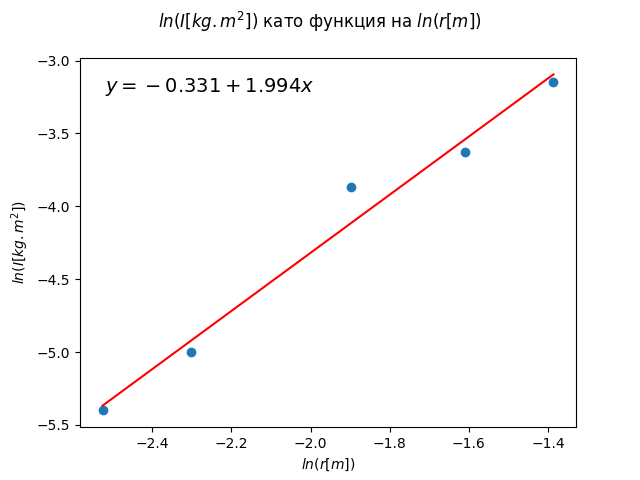
\includegraphics[width=\columnwidth, keepaspectratio=true]{graph.png}
\end{figure}

Наклонът на правата е определен като $b=1.994$, което е достатъчно близо до очакваната стойност $b=2$. Това значи, че експериментът е в съгласие с теоремата на Щайнер.  

\end{document}